\documentclass[10pt,a4paper]{article}
\usepackage[utf8]{inputenc}
\usepackage{amsmath}
\usepackage{amsfonts}
\usepackage{amssymb}
\usepackage{graphicx}
\usepackage{caption}
\author{Antonin Garret et Raphael Truffet}
\title{Projet : Ants vs SomeBees}
\date{}
\renewcommand{\contentsname}{Sommaire}

\begin{document}

\maketitle
\tableofcontents
\newpage

\section*{Introduction}

Dans ce projet, nous avons programmé un jeu intitulé "Ants vs SomeBees", inspiré du jeu "Plants vs Zombies". L'intérêt principal de ce projet était de découvrir la programmation orientée objet. Cela nous a donc amené à faire des choix de programmation de façon à exploiter au maximum cet aspect là.

\section{Dépendances entre classes}
\subsection{Diagramme de classes}

\begin{center}
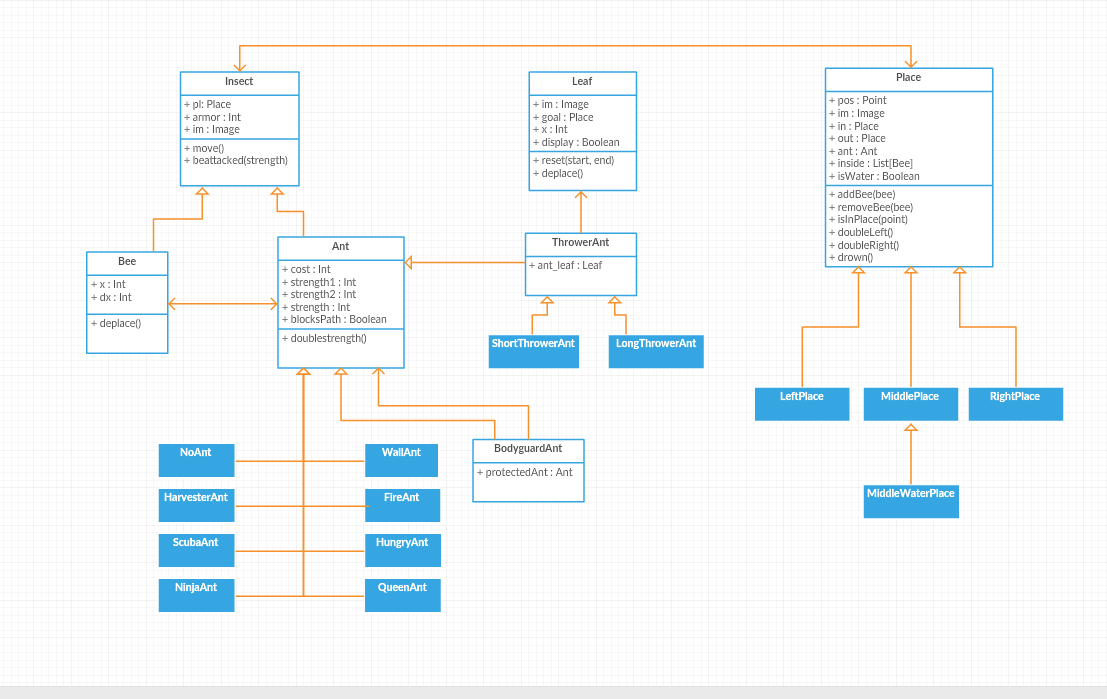
\includegraphics[scale=0.3]{ClassDiagram}
\captionof{figure}{Diagramme UML}
\label{ClassDiagram}
\end{center}

Le diagramme est également en annexe dans un format plus adapté

\subsection{Commentaires}

La programmation orientée objet a bien entendu ses avantages, comme par exemple le fait que les informations sur un objet soient regroupées. Cependant, cela peut également amener à des situations particulières, par exemple, on peut remarquer que la classe Ants contient un champ qui indique la place où se trouve la fourmi (en héritage de la classe Insect) mais aussi que la classe Place contient un champ qui indique quelle fourmi s'y trouve. L'information est donc stockée en double. On y perd lors de la création et des modifications de l'information, mais on y gagne en clarté du code et en rapidité lorsque l'on souhaite seulement accéder aux informations, ce qui est plus fréquent.

L'héritage entre les classes a permit de factoriser un bonne partie du code et de limiter la taille des pattern matching.

\section{Graphisme}

\subsection{Affichage}

Ici encore, la notion de classes a été pratique. En effet, chaque classe contenait un champ qui stocke son image. Dès lors, il suffit de parcourir tous les objets et de placer l'image à sa position (pour les insectes, la position est connue à travers le champs de place). 

\subsection{Animation fluide}
  
Le jeu se jeu au tour par tour, alors que les animations sont continues (pour les feuilles et les abeilles). Il a donc fallu gérer cette contradiction. L'idée a été de rajouté pour ces objets un champ pour indiquer sa position qui est mis à jour à chaque frame. Cette position n'est modifiée que si l'objet doit se déplacer, or cette information n'est modifiée que lorsque l'on change de tour. Dès lors, on utilise un champ qui indique la distance qu'il reste à parcourir, qui est augmenté lorsqu'un déplacement est commandé, et diminué lorsque l'objet se déplace effectivement.

\section{Interactions avec l'utilisateur}

\end{document}